 \documentclass[11pt,a4paper]{article}
\usepackage[utf8]{inputenc}
\usepackage[slovene]{babel}
\usepackage{physics}
\usepackage{amsmath}
\usepackage{bm}
\usepackage{amsfonts}
\usepackage{amssymb}
\usepackage[left=3cm,right=3cm,top=3cm,bottom=3.8cm]{geometry}
\usepackage{caption}
\usepackage{subcaption}
\usepackage{graphicx}
\usepackage{float}
\setlength\parindent{0pt}


\title{02-Airbounce: Ideje in rešitve}
\date{}

\begin{document}

\maketitle

\section{Stabilen frizbi}
Frizbi zaradi vrtenja ohranja orientacijo.

\begin{figure}[H]
	\centering
	\begin{minipage}{.5\textwidth}
	  \centering
	  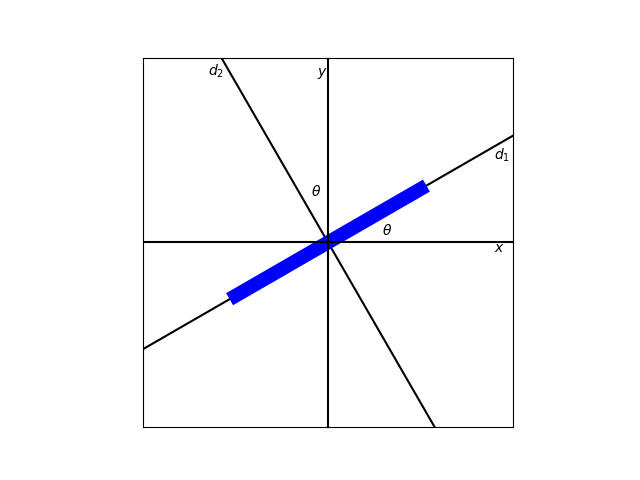
\includegraphics[width=9cm]{graf_osi.png}
	  \captionof{figure}{Graf osi, koordinatni sistem N}
	\end{minipage}%
	\begin{minipage}{.5\textwidth}
	  \centering
	  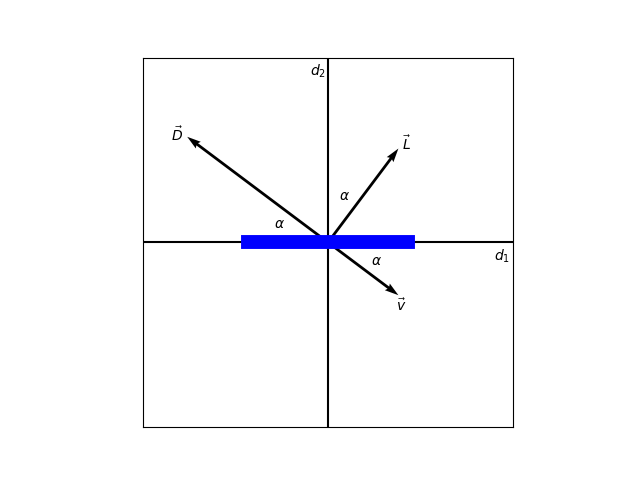
\includegraphics[width=9cm]{osi_frisbeeja.png}
	  \captionof{figure}{Koordinatni sistem frizbija D}
	\end{minipage}
	\end{figure}

V sistemu frizbija (D):
\begin{gather}
L = \dfrac{1}{2} A \rho C_L v^2 \qquad D = \dfrac{1}{2} A \rho C_D v^2\\
C_L = C_{L0} + C_{L \alpha} \alpha \qquad C_D = C_{D0} + C_{D \alpha} \alpha^2\\
K = \dfrac{A \rho}{2 m} \qquad \tan \alpha = \dfrac{-v_2}{v_1}\\
\bm L = m K v^2 C_L \mqty(\sin \alpha \\ \cos \alpha) = m K v^2 C_L \mqty(-v_2 \\ v_1\\)\\
\bm D = m K v^2 C_D \mqty(-\cos \alpha \\ \sin \alpha) = m K v^2 C_D \mqty(-v_1 \\ -v_2\\)\\
\bm F_{\bm g} = - m g  \mqty(-\sin \theta \\ \cos \theta)\\
\end{gather}

\begin{gather}
m \bm a = \bm L + \bm D + \bm F_{\bm g}\\
v = \sqrt{v_1^2 + v_2^2}\\
a_1 = -K (C_{L0} + C_{L \alpha} \alpha) v v_2 - K (C_{D0} + C_{D \alpha} \alpha^2) v v_1 - g \sin \theta\\
a_2 = K (C_{L0} + C_{L \alpha} \alpha) v v_1 - K (C_{D0} + C_{D \alpha} \alpha^2) v v_2 - g \cos\theta
\end{gather}
Rešimo: \(d_1, d_2, v_1, v_2 \).\\
Zarotiramo v N sistem.
\begin{gather}
R = \mqty(\cos \theta & -\sin \theta \\ \sin \theta & \cos \theta)\\
\mqty(x \\ y)_N = R \mqty(d_1 \\ d_2)_D\\
\mqty(v_x \\ v_y)_N = R \mqty(v_1 \\ v_2)_D
\end{gather}

\end{document}
